\outline{1}{Learning, Not Recovery, is Modulated by Joint Synergies and Redundancy Exploration in Robotic Training Post-Stroke}
\chapter{Learning, Not Recovery, is Modulated by Joint Synergies and Redundancy Exploration in Robotic Training Post-Stroke}
\label{cha:armeospring}



\outline{2}{Introduction}
\section{Introduction}



\outline{2}{Methods}
\section{Methods}

\subsection{Data Collection}

\textbf{Participants.} 
We recruited 11 young (age 23 $\pm$ 2) healthy subjects (7 males) as the control group.
We recruited 53 post-stroke individuals with gender and affected side balanced, shown in table \ref{tab:demog}. 
Participants receive conventional rehabilitation besides robot-aided rehabilitation.

\begin{table}[b]
	\begin{tabular}{c c c c c c c c}
		\hline
		Group & No. & Age & Affected Side & Gender & FM(0-66) & Post Stroke Days & No. of Tests\\
		\hline
		Stroke & 53 & 59$\pm$14 & 29L, 24R & 19F, 30M & 25$\pm$9 to 39$\pm$ 14 & 56$\pm$21 & 80 in 4 weeks \\ 
		Control & 11 & 23$\pm$2 & - & 4F, 7M & - & - & 20 in 1 weeks \\
		\hline
	\end{tabular}
	\caption{Participants information}
	\label{tab:demog}
\end{table}

\textbf{Device.}
Our robot-aided rehabilitation uses ArmeoSpring exoskeleton \cite{} for therapy training. 
Shown in figure \ref{fig:1setupschedule}, the exoskeleton has 6 degrees of freedom, summarized in table \ref{tab:devicedof}. 
It is attached to the arm by two or three velcro straps. 
The exoskeleton has two springs equipped, at the upper arm and the forearm respectively. 
The springs can be adjusted to compensate the gravity force of the arm. 
Lengths of the exoskeleton are also adjustable to adapt to user's arm length.
There are no motors at any joints, user has to move actively to control the exoskeleton. 
User's trunk is mildly constrained by the velcro strap at the upper arm.


\begin{table}
	\begin{tabular}{c c c c}
		\hline
		Joint No. & Joint Name & Anatomical Counterpart & Direction \\
		\hline
		1(a) & Inner Shoulder Angle & Shoulder Horizontal Ab-/Adduction & Left/Right \\
		1(b) & Outer Shoulder Angle & Shoulder Horizontal Ab-/Adduction & Left/Right \\
		2 & Upper Arm Angle & Shoulder Flex-/Extension & Up/Down \\
		3 & Elbow Angle & - & Left/Right \\
		4 & Forearm Angle & - & Up/Down \\
		5 & Pro-/Supination Angle & Pro-/Supination & - \\ 
		6 & Flex-/Extension Angle & Wrist Flex-/Extension & - \\
		\hline
	\end{tabular}
	\caption{Degrees of freedom of ArmeoSpring exoskeleton.}
	\label{tab:devicedof}
\end{table}

The device records all joint angles (that is, the joints of the exoskeleton), and calculates the end effector location through a forward kinematics model of the exoskeleton. 
The end effector location then is used to control a cursor on a screen, displayed vertically in front of the user. 
All joint angles and end effector locations are recorded.

\textbf{Training and Test.}
Participants in the control group receive two training sessions (morning and afternoon) for five consecutive days in a week.
Post-stroke participants receive the same amount of training per day every weekday for 4 consecutive weeks (Figure \ref{fig:1setupschedule} C).

One training session consists of several games, each lasts at most 3 minutes (with the exception of the ladybug pointing test mentioned below); after a certain game, the user is often presented with performance feedbacks of that game. 
One training session typically lasts about 20 minutes for young healthy adults.

A ladybug pointing test is scheduled at the beginning and the end of each training session. 
In this test, the user tries to catch ladybugs that appear one by one pseudo randomly on a vertical screen in front of the user. 
The sequence of locations that ladybugs appear are fixed, although within a test they seem random.
The game is two-dimensional; the movement along the dimension perpendicular to the screen is ignored. 
To catch the ladybug, the user moves the cursor to its location. 
The user has limited time to catch the ladybug.
After a ladybug is caught, or time limit is reached, the ladybug disappears and the next ladybug appears somewhere else. 

\subsection{Data Analysis}

\textbf{Preprocessing.}
We filter the data with a second order Butterworth filter with a cutoff frequency of 5 Hz.
We define a trial as the movements between two consecutive ladybugs.
A trial is considered successful if it starts from previously caught target and leads to the catching of next target.

\textbf{Task Space Performance.}
We characterize task space performance via number of peaks in the velocity profile \cite{}.
For participants in the control group, we model the number of peaks ($ p $) with an exponential model
\begin{equation}\label{eqn:singleexp}
p = a e^{-b t} + 1
\end{equation}
where $ t $ is test number, $ b $ is learning rate.
We choose an asymptote of 1 because it is the theoretical limit of number of peaks.

For participants in the stroke group, we assume that two components are necessary to model the number of peaks
\begin{equation}\label{eqn:doubleexp}
p = a_1 e^{-b_1 t} + a_2 e^{-b_2 t} + 1
\end{equation}
$ a_1, a_2, b_1 $ and $ b_2 $ are constraint to be positive.
We fit a nonlinear mixed effect model \cite{} to equation \ref{eqn:singleexp} and \ref{eqn:doubleexp} via Matlab 2016a function \textsf{nlmefit}.
The results of mixed effect model include the fixed effect $ \hat{a} $ and $ \hat{b} $ that represents group average, and the random effect for each participant $ a_s $ and $ b_s, s = 1, ..., N_\text{sb} $.

\textbf{Joint Space Variability.}
To quantify joint space variability and its relevance to the task space, we use a nonlinear forward kinematics model of the exoskeleton (cite company?)
	\begin{equation}\label{eqn:nonlinearForwardKinematics}
	\bm{r} = f(\bm{\theta})
	\end{equation}
where $ \bm{r} = (x,y)^T $ is the location of the end effector, $ \bm{\theta} $ is joint angles (see table \ref{tab:devicedof} for details). 
The distribution of variability is calculated for the last 10 tests at the moment of catching ladybugs. 
The mean joint configuration at one specific ladybug ($ b $) is denoted by $ \bar{\bm{\theta}}_b $.
We will omit index $ b $ for convenience.
The Jacobian matrix at configuration $ \bar{\bm{\theta}} $ is obtained through forward kinematics (equation \ref{eqn:nonlinearForwardKinematics})
	\begin{equation}
	\bm{J}(\bar{\bm{\theta}}) = \frac{\partial f(\bm{\theta})}{\partial \bm{\theta}} \Big\rvert_{\bar{\bm{\theta}}}
	\end{equation}
and $ \bm{J} $ is a 2 by 6 matrix.
The null space of Jacobian $ \bm{J} $ can be represented by basis of the space $ \bm{\xi}_i $, $ i= 1,2,3,4 $ which satisfy
	\begin{equation}
	\bm{J}(\bar{\bm{\theta}}) \bm{\xi}_i = 0
	\end{equation}
For a specific trial, the deviation of joint angles from $ \bar{\bm{\theta}} $ is
	\begin{equation}
	\Delta\bm{\theta} = \bm{\theta} - \bar{\bm{\theta}}
	\end{equation}
The projection of $ \Delta\bm{\theta} $ to the null space is
	\begin{equation}
	\Delta\bm{\theta}_{\text{null}} = \sum_i^m \langle \Delta\bm{\theta}, \bm{\xi}_i \rangle \bm{\xi}_i, m=4
	\end{equation}
In the end, we quantify the null space variability by calculating the mean of squared $ \Delta\bm{\theta}_{\text{null}} $
	\begin{equation}
	V_{\text{null}} = \mathbb{E}_{t,b} (\Delta\bm{\theta}_{\text{null}}^T\Delta\bm{\theta}_{\text{null}})
	\end{equation}
where $ t,b $ index tests and targets (ladybugs).

To obtain variability in the orthogonal space, we simply replace $ \bm{\xi}_i $ with the basis of the orthogonal space, $ \bm{\psi}_i $, $ i= 1,2 $  :
	\begin{equation}
	\Delta\bm{\theta}_{\text{orth}} = \sum_i^m \langle \Delta\bm{\theta}, \bm{\psi}_i \rangle \bm{\psi}_i, m=2
	\end{equation}
and the orthogonal space variability is
	\begin{equation}
	V_{\text{orth}} = \mathbb{E}_{t,b} (\Delta\bm{\theta}_{\text{orth}}^T\Delta\bm{\theta}_{\text{orth}})
	\end{equation}

\textbf{Synergy Extraction and Analysis.}
We use Principal Component Analysis (PCA) to extract joint synergies from each ladybug test. 
In this study, we only look at the first two synergies.
On average, the first two synergies account for 83.9\% joint angle variance for control group, 83.1\% for stroke group.
Joint synergies of healthy participants are quite stable across individuals.
We calculate the averaged synergies shown in figure \ref{fig:6synergy}-C.
To measure the synergy pattern of stroke participant, we use the Dihedral angle between subspaces that are spanned by synergies \cite{}.

Specifically, given two $ 4 \times 2 $ matrices representing two sets of synergies (or subspaces) $ U $ and $ V $, the Dihedral angle between them is defined as
	\begin{equation}\label{eqn:dihedral}
	\phi(U,V) = \arccos(s_\text{min}(U^TV))
	\end{equation}
where $ s_\text{min}(U^TV) $ represents the minimum singular value of matrix $ U^TV $.

We investigate this Dihedral angle between the average healthy synergies and synergies of stroke participants from every test.

We fit a linear mixed effect model to this angle with a random effect on the intercept.

We then correlate this intercept with 


\outline{2}{Results}
\section{Results}

\textbf{Task Space Performance.}
Figure \ref{fig:nopcontrol} shows the number of peaks modeled by a single exponential function.

\outline{2}{Discussion}
\section{Discussion}



\begin{figure}
	\centering
	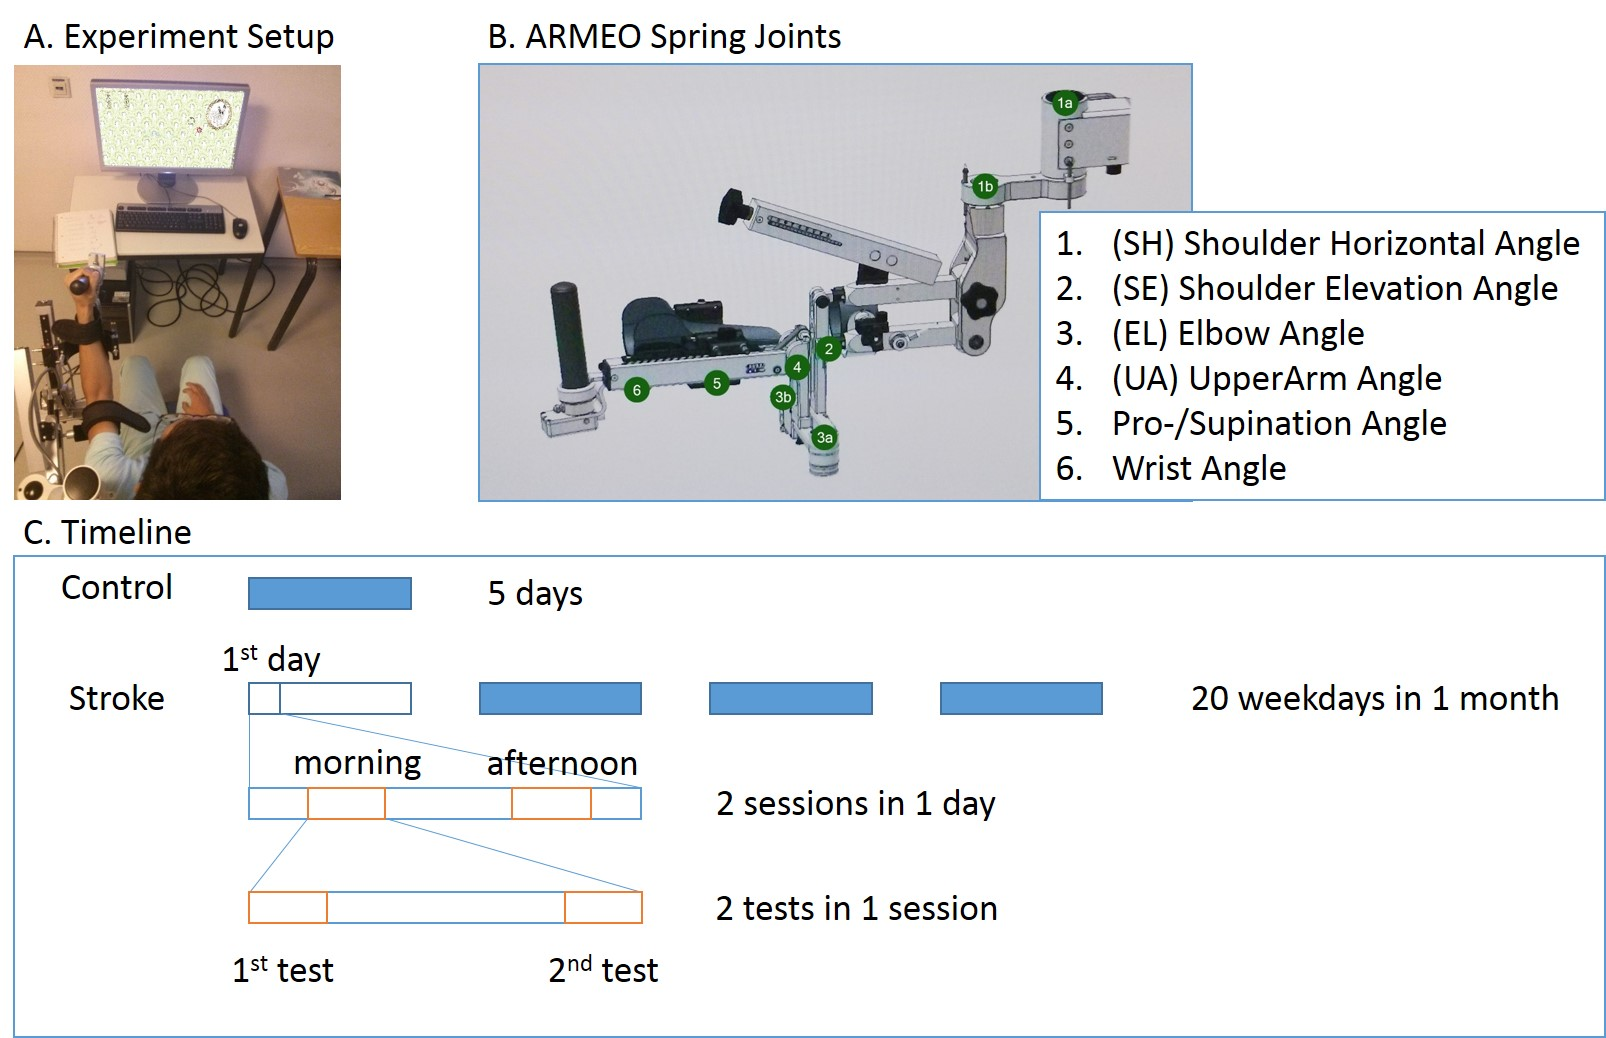
\includegraphics[width=1\linewidth]{figures/1setup&schedule}
	\caption[Experiment Setup and Schedule]
	{Experiment Setup, ARMEO Spring and Schedule. 
		A: Participants sit in front of a vertical screen on which the training games are displayed. In the ladybug test, the cursor responds to movements on a vertical plane. 
		B: Joints of ARMEO Spring. Summation of 1a and 1b is Shoulder Horizontal (SH) angle; 2 is Shoulder Elevation (SE) angle; 3a (only activated for right arm) and 3b (left arm) are elbow (EL) angles; 4 is ForeArm (FA) angle; 5 is pronation and supination angle; 6 is wrist angle.
		C: Two ladybug tests are administered at beginning and end of one session, two sessions are administered in morning and afternoon. Control group receives 5 days training, whereas stroke group receives 20 consecutive weekdays training.}
	\label{fig:1setupschedule}
\end{figure}

\begin{figure}
	\centering
	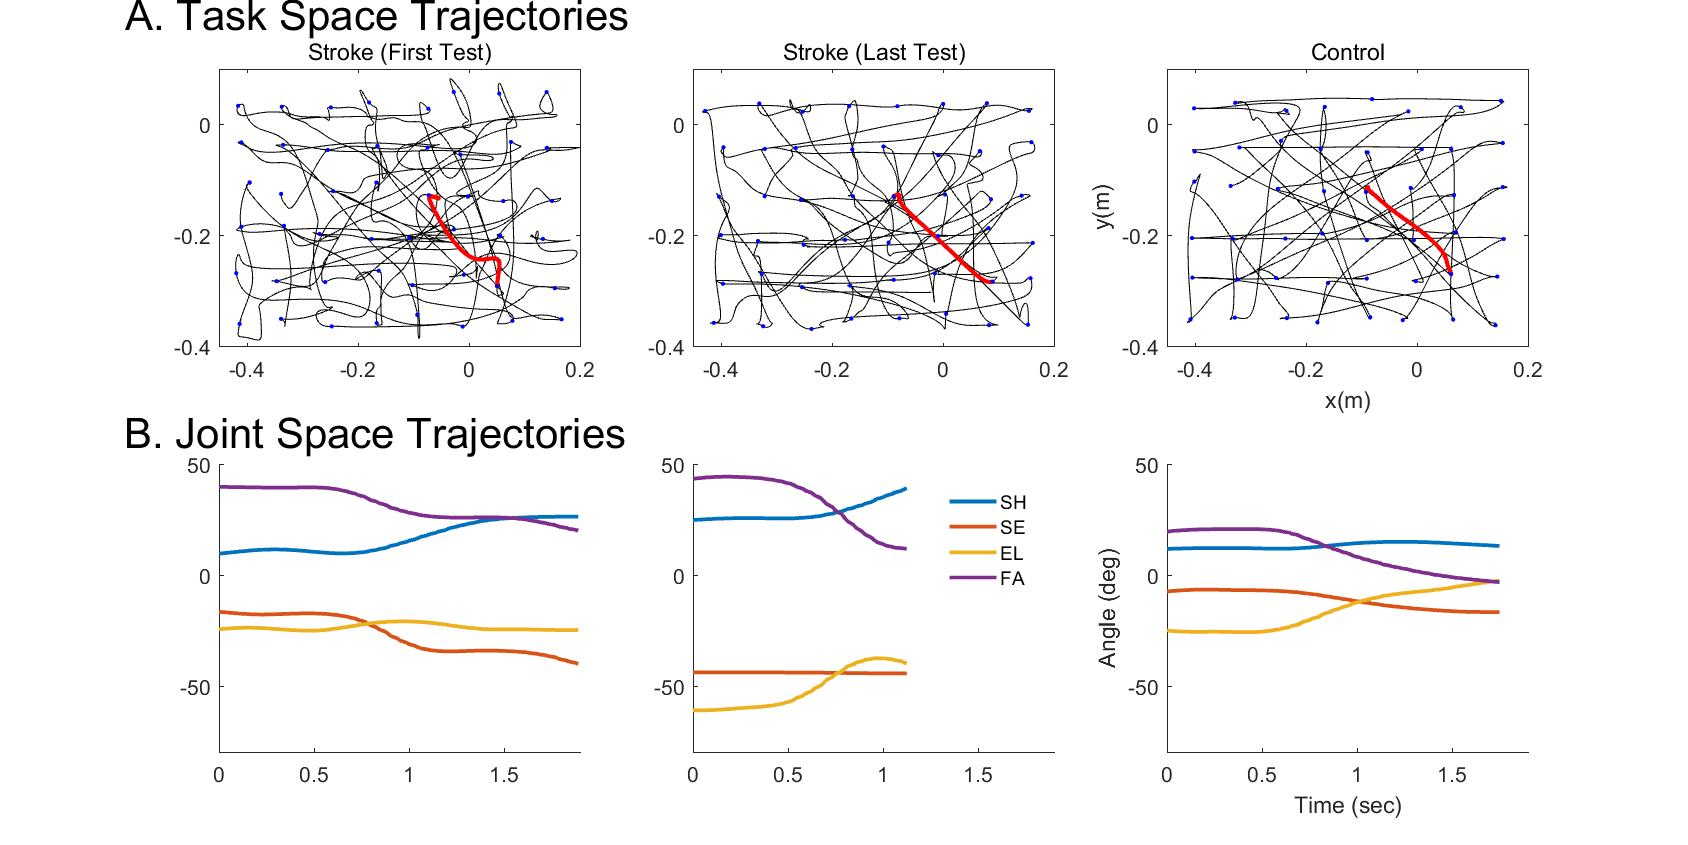
\includegraphics[width=1\linewidth]{figures/2strokeTrajExamp}
	\caption[Example trajectories]
	{Representative trajectories. 
		Top row: example cursor trajectories.
		Bottom row: example joint angle trajectories. Only the first four joints are shown.}
	\label{fig:2stroketrajexamp}
\end{figure}


\begin{figure}
	\centering
	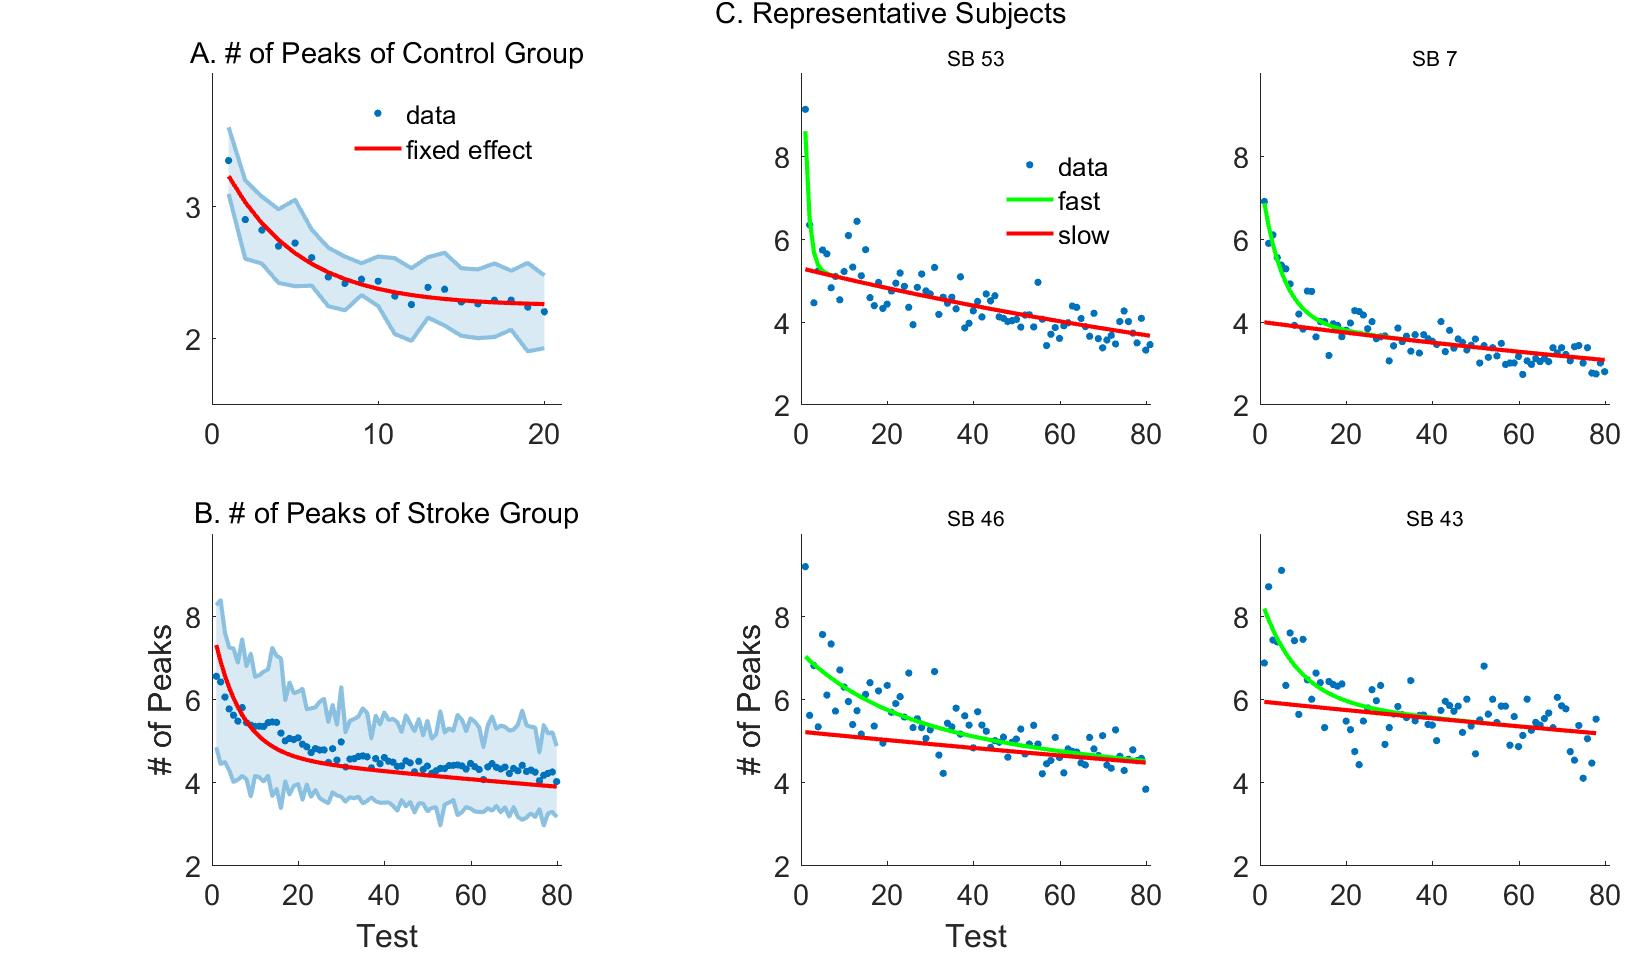
\includegraphics[width=1\linewidth]{figures/3nopFixRan}
	\caption[Double Exponential Model]
	{Double Exponential Model of Number of Peaks in Velocity Profile. 
		A,B: The fixed effect
		C: representative participants who show fast learning rate and large null variability,..
		D: }
	\label{fig:3nopfixran}
\end{figure}

\begin{figure}
	\centering
	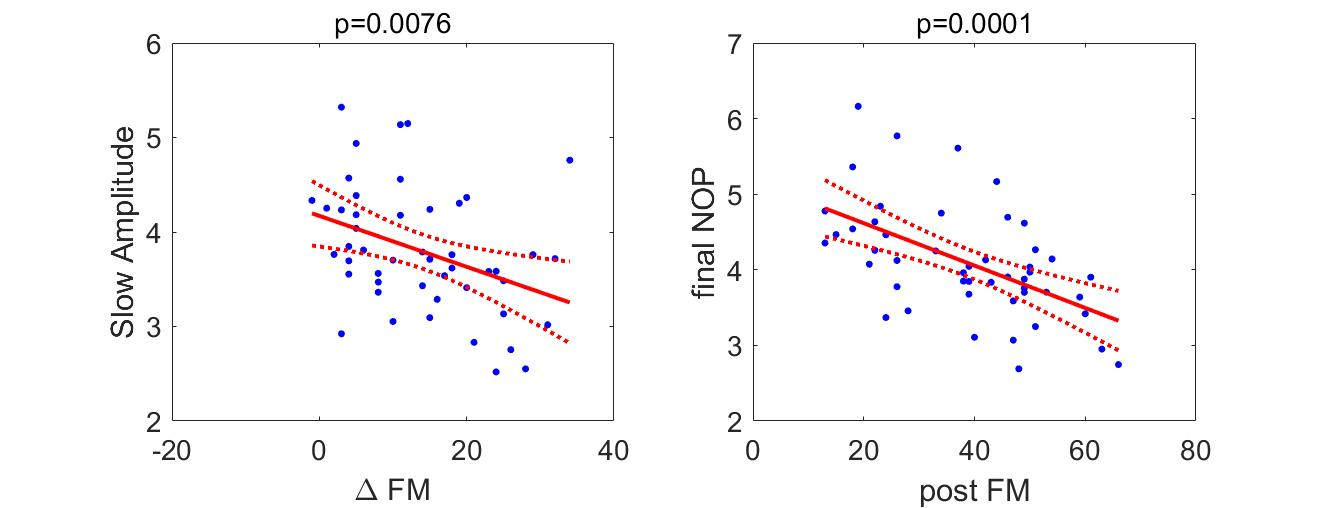
\includegraphics[width=1\linewidth]{figures/4slowComponentIsRecovery}
	\caption[Slow component corresponds to recovery as meaured by FM]
	{Slow component corresponds to recovery as meaured by FM. 
		A: The number of peaks post training is correlated with FM post training;
		B: The change of number of peaks is correlated with the change of FM, prior and post training.}
	\label{fig:4slowcomponentisrecovery}
\end{figure}

\begin{figure}
	\centering
	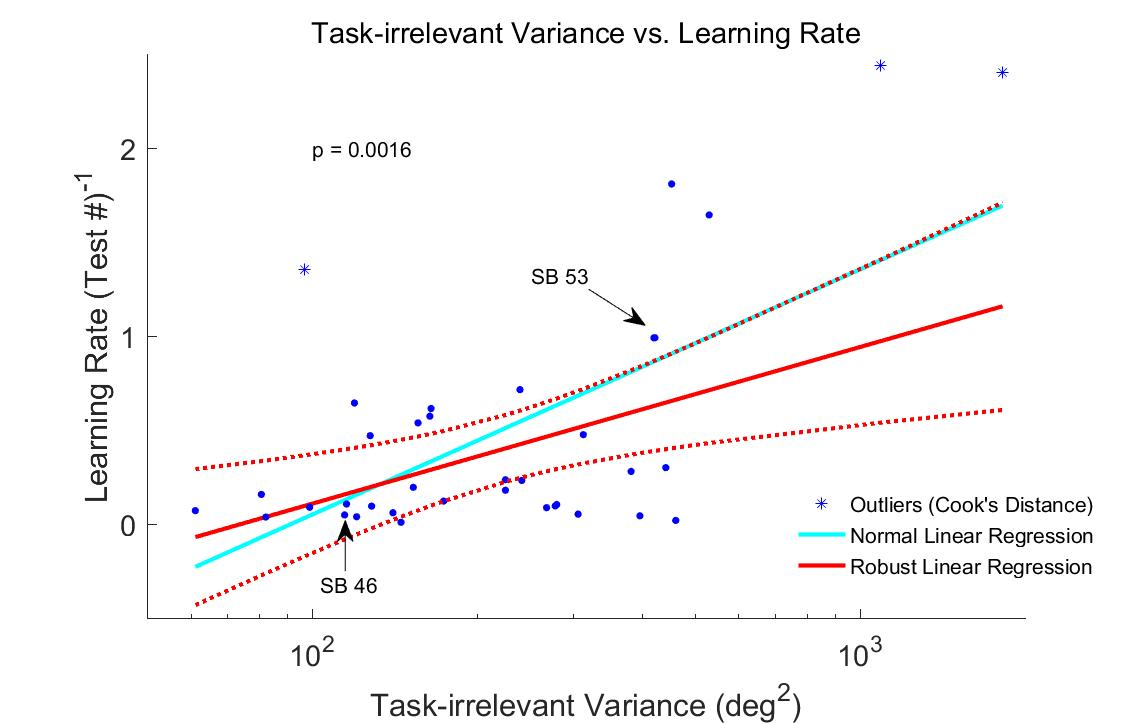
\includegraphics[width=1\linewidth]{figures/5learnRateVSnullVar}
	\caption[Exploration of Joint Redundancy facilitates learning]
	{Exploration of Joint Redundancy facilitates learning. (The log of) null space variability is correlated with learning rate}
	\label{fig:5learnratevsnullvar}
\end{figure}

\begin{figure}
	\centering
	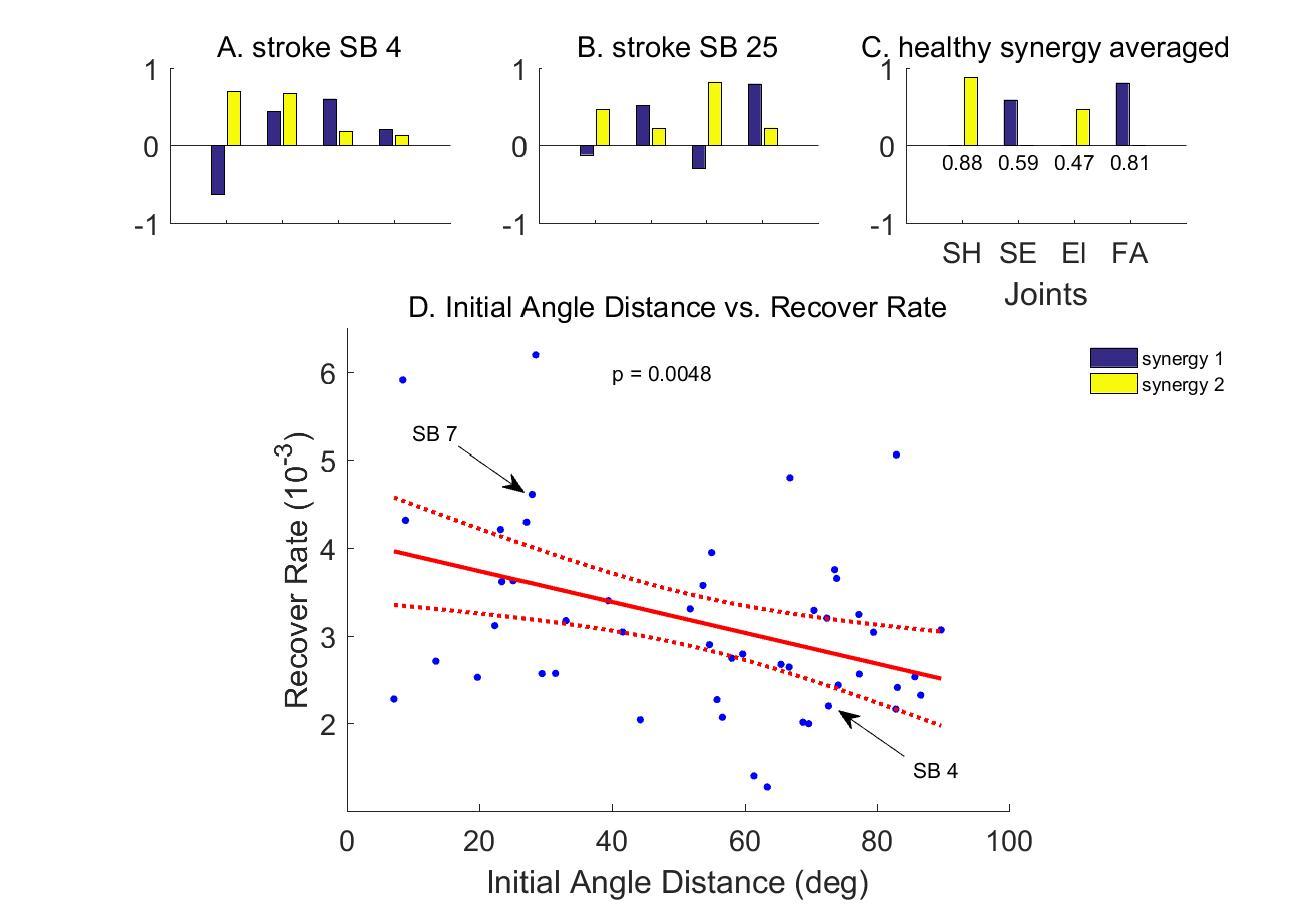
\includegraphics[width=1\linewidth]{figures/6synergy}
	\caption[Abnormal Synergies]{}
	\label{fig:6synergy}
\end{figure}

